\chapter{Rapid and Robust Spin Amplification} 
\label{ch:SpinAmplification}


The standard approach to implementing a quantum technology is to identify a physical system that can represent a qubit: it must exhibit two (or more) stable states, it should be manipulable through external fields and possess a long decoherence time. Provided that the system can controllably interact with other such systems, then it may be a strong candidate. Electron and nuclear spins, within suitable molecules or solid state structures, can meet these requirements. However the drawback with spin qubits is that they have not been directly measured through a detection of the magnetic field they produce. The magnetic moment of a single electron spin is orders of magnitude too weak to be detected by standard ESR techniques and even the most sensitive magnetometers still fall short of single spin measurement~\cite{cleuziou06} - meanwhile the situation with nuclear spins is worse still. In a few special systems it is possible to convert the spin information into another degree of freedom. For example, a spin-dependent optical transition allow spin to photon conversion in some crystal defects~\cite{nv_oscillation_04, neumann10, morello_spin_readout_10}, self-assembled semiconductor quantum dots~\cite{vamivakas10, Berezovsky:2008p6616}, and trapped atoms held in a vacuum~\cite{leibfried03}. Alternatively, spin to charge conversion is an established technology in lithographic quantum dots~\cite{quantum_dot_review_07}. However, the majority of otherwise promising spin systems do not have such a convenient property~\cite{morton10} and therefore cannot be measured directly.

One suggested solution is to `amplify' a single spin, by using a set of ancillary spins that are (ideally) initialised to $\ket{0}$. We would look for a transformation of the form
\begin{equation}
  \ket{0}\ket{0}^{\otimes n} \rightarrow \ket{0}\ket{0}^{\otimes n} \ \ \ \ \ \
  \ket{1}\ket{0}^{\otimes n} \rightarrow \ket{1}\ket{1}^{\otimes n},
\end{equation}
the idea being that the $n$ ancillary spins constitute a large enough set that state of the art magnetic field sensing technologies can detect them. Note that the transformation need not be unitary or indeed even coherent: since the intention is to make a measurement of the primary spin, it is not necessary to preserve any superposition (that is, we need not limit ourselves to transformations that take $\alpha\ket{0}\ket{0}^{\otimes n} +\beta\ket{1}\ket{0}^{\otimes n} $ to a cat state like $\alpha\ket{0}^{\otimes n+1}+\beta\ket{1}^{\otimes n+1}$).  

This is a rather broadly defined transformation and there are a number of ways that one might perform it. Clearly one would like to find the method that is the least demanding experimentally. Previous authors have proposed schemes using a strictly one-dimensional (1D) homogeneous lattice with continuous global driving \cite{Lee:2005p6468}, and an inhomogeneous three-dimensional (3D) lattice with alternating timed EM pulses \cite{PerezDelgado:2006p6542}. The former result has the advantage of simplicity but the rate at which amplification occurs will inevitably be limited by the single dimension of the array; moreover such a system must be highly vulnerable to imperfect initialisation (i.e. finite temperature).

In this chapter we present an amplification procedure using a homogeneous two-dimensional (2D) square lattice. We show that a continuous global EM field can drive an amplification process that succeeds at finite temperatures (imperfect initialisation of the ancilla spins) and in the presence of decoherence. By bringing the global EM field onto resonance with certain transitions, we are able to create a set of rules that govern locally how spins propagate over the lattice. We then look at the rate of increase in the total number of flipped spins as a measure of quality of the scheme. While our focus is on the 2D case, we are also able to predict the performance of the amplification protocol for a homogeneous 3D lattice with continuous driving.

\section{Review of 1D Model}

The case of a 1D lattice has been studied in detail by Lee and Khitrin \cite{Lee:2005p6468}. Before moving to the 2D spin lattice that will form the core of the chapter, we first recall how to simplify the description of this (semi-infinite) 1D spin chain, with nearest neighbour Ising (ZZ) interactions. Under a microwave driving field of frequency $\omega$, the Hamiltonian is given by
\begin{equation} {\cal H} = \sum_{i=1}^{\infty} \epsilon_i \sigma^i_z
  + J_i \sigma_z^i\sigma_z^{i+1} + 2 \Omega_i \sigma_x^i \cos(\omega
  t)
\end{equation}
$\epsilon_i$ is the on-site Zeeman energy of spin $i$, and $J_i$ is the magnitude of the coupling between spins $i$ and $i+1$. $\Omega$ describes the coupling of spin $i$ and the microwave field. In this case, spin $i=1$ is the one whose state is supposed to be amplified. We assume that the chain is uniform, such that $\Omega_i = \Omega$, $\epsilon_i = \epsilon$ and $J_i = J$, and that $\Omega$ is weak. Following the same procedure as in Section~\ref{semiclassical_atom_cavity}, we move into a frame rotating at frequency $\omega$ and make a rotating wave approximation, setting $\omega = \epsilon$:
\begin{equation} {\cal H} = \sum_{i=1}^{\infty} J
  \sigma_z^i\sigma_z^{i+1} + \Omega \sigma_x^i .
\end{equation}
In order to understand the dynamics of the system, is it instructive to explicitly separate all terms that involve a particular spin $k$:
\begin{equation} {\cal H} = J (\sigma_z^{k-1} +
  \sigma_z^{k+1})\sigma_z^k + \Omega \sigma^k_x + \sum_{i \neq \{k,
  k-1\}} \Omega\sigma_x^i + J \sigma_z^i\sigma_z^{i+1} +
  \Omega\sigma_x^{k-1}
  \label{hamk}
\end{equation}
Choosing a driving field such that $\Omega\ll J$ means that spin $k$ will only undergo resonant oscillations when the first term in Eq.~\ref{hamk} goes to zero - i.e. when the two spins neighbouring spin $k$ are oriented in opposite directions. In any other configuration the Ising coupling takes the spin $k$ off resonance with the microwave and no appreciable dynamics are expected.

\begin{figure}[htb]
  \begin{center}
    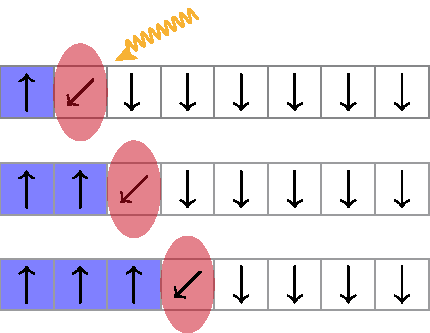
\includegraphics{figures/1D_spin_lattice.pdf}
  \end{center}
  \caption{States of the 1D chain: only spins with one neighbour $\uparrow$ and the other neighbour $\downarrow$ are on resonance.}
  \label{1D_spin_lattice}
\end{figure}

Let us now define a subset of states $S$ that exist in the spin chain Hilbert space, $\ket{n}$, which have the first $n$ spins of the chain in state $\ket{\uparrow}$ with the rest $\ket{\downarrow}$. If the rule we just derived holds exactly, these states define a closed subspace. We may then write a very simple isolated Hamiltonian for this subspace:
\begin{equation}
  {\cal H}_S = \Omega \sum_{n=1}^\infty \ket{n}\bra{ n+1}+\ket{n+1}\bra{ n}.
  \label{1d_ham}
\end{equation}
The Hamiltonian couples states with $n$ up-spins to those with $n-1$ and $n+1$, with coupling strength $\Omega$. 

\section{Extension to 2D Model}

With this simplification of the 1D Hamiltonian in mind, we progress now to a semi-infinite square spin lattice with nearest-neighbour ZZ interactions. For this case we have
\begin{equation} {\cal H} = \sum_{i=1}^{\infty}\sum_{j=1}^\infty
  \epsilon \sigma^{i, j}_z + J \sigma_z^{i, j}\sigma_z^{i+1, j} +
  J\sigma_z^{i, j}\sigma_z^{i, j+1} + 2 \Omega \sigma_x^{i, j}
  \cos(\omega t).
\end{equation}
By again considering the terms affecting a particular spin in the main body of the lattice ($k(>1), l(>1)$ say) we find for $\omega = \epsilon$ and after moving to a rotating frame and making the rotating wave approximation:
\begin{equation}
  {\cal H} = J \sigma_z^{k, l} (\sigma_z^{k+1, l} + \sigma_z^{k, l+1} + \sigma_z^{k-1, l} + \sigma_z^{k, l-1}) +...
\end{equation}
where we do not explicitly write out terms not involving spin $(k, l)$.  The microwave is now only resonant for spin $(k, l)$ if it has two neighbour spins in each orientation. For a spin on the edge of the lattice there are an odd number of neighbours so resonance cannot be achieved in this case. However, applying a second microwave with $\omega = \epsilon - J$ allows resonant flips on the edge if two neighbours are down and one up - and this second field has no effect on the bulk spins.

The spin to be measured is the corner spin ($i=j=1$) and so would form part of a wider computational apparatus. We may therefore assume that it is a different species with a unique resonant frequency. The dynamics of the whole lattice may then be summarised by three rules (in order of precedence):
\begin{enumerate}
  \item The corner (test) spin is fixed.\vspace{-0.2cm}
  \item An edge spin can flip if it has one of its neighbours up and
    two down.\vspace{-0.2cm}
  \item A body spin can flip if it has two of its neighbours up and two down.\vspace{-0.2cm}
\end{enumerate}
We begin by supposing all spins are initialised in the `down' state apart from the test spin, which is located in the upper left hand corner of our lattice. We can describe this initial state by choosing two basis elements: $\ket 0$ when the test spin is down, and $\ket 1$ when the test spin is up. Using our heuristic rules we can see that these two states do not couple to each other - that $\bra 0H\ket 1=0$. In fact $\ket 0$ does not couple to any other state, so if we start in the $\ket 0$ state no amplification occurs, as desired.


\section{Building a Subspace Basis} 

We will now seek to construct a basis for the subspace containing our system evolution, by looking at states connected by our Hamiltonian. It will be convenient to represent these states on the nodes of a graph, using the edges to represent non-zero elements of the Hamiltonian.

Our starting point is the state $\ket 1$, with just the corner spin `up'. From this position our rules allow two possibilities: either the spin to the right of the corner flips, or the spin below it flips (see Fig.~\ref{partition_states}). In each case, the magnitude of the transition matrix element is $\Omega$. As we continue this procedure, we notice that the states that arise for each excitation number can be characterised by a non-increasing sequence of integers that represent the number of `up'-spins in each column of the lattice (see Fig.~\ref{partition_states}). Such sequences can also be used to define partitions of at integer: ways of splitting an integer up into a sum of other integers, e.g. $3=3=2+1=1+1+1$. In fact, the states that arise are in 1-to-1 correspondence with such partitions; we call these states `partition states' and denote them with standard partition notation (see Fig.~\ref{partition_states}).
\begin{figure}
  \begin{center}
    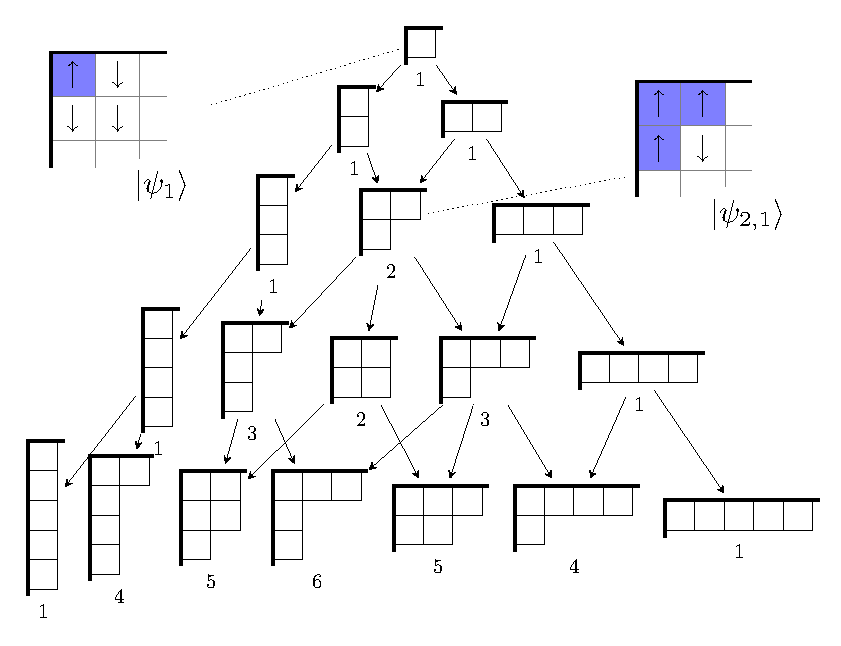
\includegraphics[scale=0.8]{assets/youngs_lattice_with_spins}
  \end{center}
  \caption{Partition states arranged into a lattice. Edges represent a coupling
    through the Hamiltion of strength $\Omega$. Weights represent the
  number of different paths through the lattice to a given state.}
  \label{partition_states}
\end{figure}
The graph we have just described is depicted in Fig.~\ref{partition_states}  is known as `Young's lattice' and arises in areas of pure mathematics, such as the representation theory of the symmetric group, and the theory of differential posets \cite{Sagan:2001p6568}. We have drawn weights beneath each state, recording the number of ways the state can be constructed. We will now further reduce the dimension of this basis
by eliminating combinations of states which are inaccessible.

Starting with $\ket 1$ we see that $\bra 1H\left(\alpha_{1,1}\ket{\psi_{1,1}}+ \alpha_{2}\ket{\psi_{2}}\right) =\Omega\left(\alpha_{1,1}+ \alpha_{2}\right)$ so $\ket 1$ does not couple to the two-excitation state $\ket{\psi_{1,1}}-\ket{\psi_{2}}$. We can eliminate this, leaving a single orthogonal, coupled state with two excitations: $\ket 2 := \frac{1}{\sqrt{2}}\left( \ket{\psi_{1,1}}+\ket{\psi_2} \right)$.

We may continue to build up coupled states with larger excitation numbers, and in fact we find that there is only a single coupled state in each case (i.e. we can always eliminate $k-1$ combinations of partition states with $k$ excitations).  To see this, first suppose we have the coupled state with $k$ excitations, which by analogy with the 1D case we write as $\ket k$. We can write $\ket k=\frac{1}{N_k}\sum_{i\in P(k)}c_{i}\ket{\psi_{i}}$, where $P(k)$ is the set of partitions of the integer $k$ and $N_k$ a normalisation factor. We want to construct the state $\ket{k+1}$ by eliminating the $k$-dimensional subspace with $k+1$ excitations, to which $\ket{k}$ does not couple.

Let $\ket{\psi}=\sum_{j\in P(k+1)}\alpha_{j}\ket{\psi_{j}}$ and consider the states $\ket{\psi}$ such that \[ 0=\bra kH\ket{\psi}=\sum_{i\in P(k)}\sum_{j\in P(k+1)}c_{i}^{*}\alpha_{j}\bra{\psi_{i}}H\ket{\psi_{j}}\] but $\bra{\psi_{i}}H\ket{\psi_{j}}=\Omega$ if $i$ is a {\it parent} of $j$ (a state connect to $j$, in the lattice row above it), and $0$ otherwise, so \[0=\bra kH\ket{\psi}=\sum_{j\in P(k+1)}\alpha_{j}\sum_{i\in parents(j)}c_{i}^{*}.\] This is the equation of a hyperplane in $|P(k+1)|$ dimensions, defining the states that are not coupled to $\ket k$ through the Hamiltonian.  There is a unique single state orthogonal to this hyperplane, $\beta_{j}=\sum_{i\in parents(j)}c_{i}$, to which $\ket k$ couples.  So the only state with $k+1$ `up'-spins that $\ket k$ couples has coefficients proportional to $\beta_{j}$. After normalisation, we call this state $\ket{k+1}$.

Unfortunately there is no easy way to write down the partition states and weights for the $n$th row of the lattice. Fortunately, for our purposes, we only need to know that the states $\ket k$ exist and what the coupling between them is. To find this coupling, consider
\begin{align}
  g_{n-1,n} & = \bra nH\ket{n-1} \nonumber\\
  & = \frac{1}{N_{n-1}N_n}\sum_{i\in P(n)}\sum_{j\in
  P(n-1)}c_{i}^{*}c_{j}\bra{\psi_{i}}H\ket{\psi_{j}} \nonumber\\
  & = \frac{1}{N_{n-1}N_n}\Omega\sum_{i\in P(n)}c_{i}^{*}\sum_{j\in
  parents(i)}c_{j} \nonumber\\
  & = \frac{1}{N_{n-1}N_n}\Omega\sum_{i\in P(n)}|c_{i}|^{2} =
  \Omega\frac{ N_n}{N_{n-1}}\label{coupling_as_sum_c2}\end{align}
To find the $N_n$ we need the sum of the squares of the weights of partitions in a given row. A standard result about Young's lattice immediately gives us this sum: $n!$ \cite{STANLEY:1975p6605}.

This result can be taken straight from the representation theory of the symmetric group: it can be shown that the nodes and their weights represent the irreducible representations and their dimensions. Given that the dimension of each representation is its multiplicity in the regular representation (with dimension $|S_n| = n!$), by dimension counting the result follows. However, for our purposes it is more enlightening to focus on a differetial poset approach, which uses particular combinatorial features of the lattice to produce the result. Here we give a brief overview of the approach detailed by Sagan in \cite{Sagan:2001p6568}.

Let $L$ be an operator that takes a partition state to a sum of its
children, and $R$ take a state to the sum of its parents. For example\begin{eqnarray*}
  L\ket{\psi_{1}} & = & \ket{\psi_{1,1}}+\ket{\psi_{2}}\\
  R\ket{\psi_{2,1}} & = & \ket{\psi_{1,1}}+\ket{\psi_{2}}\end{eqnarray*}
We add a state $\ket\emptyset$ such that $L\ket\emptyset=\ket{\psi_{1}}$
and $R\ket\emptyset=0$. Then
\begin{align}
  L^{n}\ket\emptyset=\sum_{i\in P(n)}c_{i}\ket{\psi_{i}}
\end{align}
and
\begin{align}
  R^{n}L^{n}\ket\emptyset=\sum_{i\in P(n)}|c_{i}|^{2}
\end{align}
We then need to use two facts about the structure of the lattice: that each element has one more child than it does parents, and each pair of elements either share both a single parent and a single child, or neither. The first of these properties is easy to see: each child corresponds to adding a square at a concave corner of the diagram, and each parent corresponds to removing a convex corner. These corners alternate along the boundary of the shape, starting and ending with concave ones, and so there is always one more child than parents.  The second property requires more work, but is roughly because two elements share a parent if, when placed on top of one another they differ by precisely two squares. Taking the union of these shapes you can find the unique child that they also both share.

These properties imply the commutation relation $RL-LR=I$, so
\begin{align}
  R^{n}L^{n}\ket\emptyset=R^{n-1}L^{n}R\ket\emptyset+nR^{n-1}L^{n-1}\ket\emptyset=...=n!\ket\emptyset
\end{align}
and so, $n!=\sum_{i\in P(n)}|c_{i}|^{2}$.

Referring back to Eq. (\ref{coupling_as_sum_c2}), and using $N_i=\sqrt{i!}$, we see that
\begin{equation}
  {\cal{H}} = \Omega \sum_{n} \sqrt{n} \left( \ket{n-1} \bra{n} +
  \ket{n} \bra{n-1} \right) .
  \label{2d_ham}
\end{equation}
In essence we have established a linear sequence of states, each coupled to the next analogously to the states on a 1D chain \ref{1d_ham}. However, each of our states is in fact a superposition of many configurations of the 2D array, and crucially the effective coupling from each state to the next increases along the sequence.

\section{Rate of Spin Propagation}

It has been shown (e.g. \cite{Fitzsimons:2005p6472}) that a quantum state released at the end of a semi-infinite chain of states, with constant couplings, will travel ballistically: the average position of the state along the chain is proportional to the time passed, and inversely proportional to the coupling strength. Since, in the one-dimensional case, the position is proportional to the number of spins that have flipped, we have that the total polarisation will increase linearly with time.

We can establish the rate of propagation in the 2D case using the ansatz that the time taken to travel between two neighbouring nodes is inversely proportional to the strength of the coupling between them. The total time is then $t_{2D}\propto \sum_{i=1}^{n}\frac{1}{\sqrt{i}}\simeq n^{\frac{1}{2}}$. As in the one-dimensional case, the position along the chain corresponds to the  number of spins that have flipped, and so we would expect the total polarisation to be proportional to $t^2$. This prediction of a quadratic speed-up of signal going from 1D to 2D is the central result of the chapter, and was confirmed by simple numerical simulations of Eq.~(\ref{2d_ham}) (Fig. \ref{comparison}).

\begin{figure}
  \begin{center}
    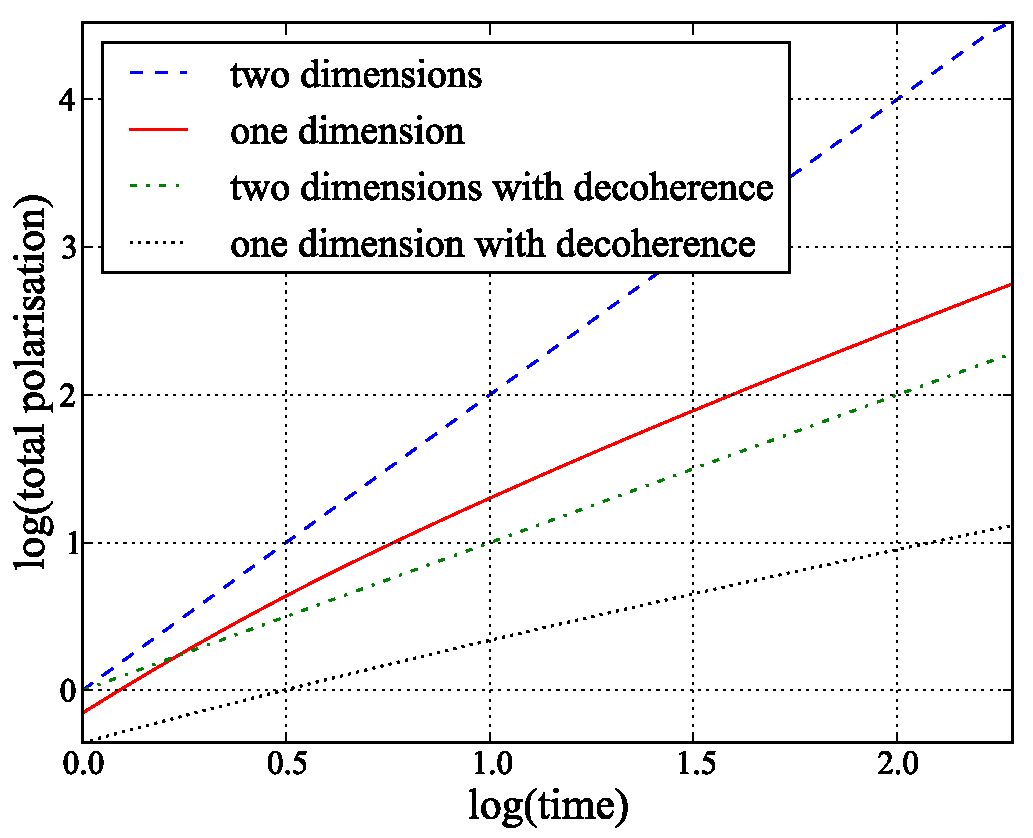
\includegraphics[scale=0.7]{assets/comparison.pdf}
  \end{center}
  \caption{Expected total polarisation against time. Time in units of $\frac{1}{\Omega}$, dephasing rate $\Gamma = 1$. The gradient of the `one dimension with decoherence' line tends to $\frac{1}{2}$ asymptotically.}
  \label{comparison}
\end{figure}

\section{Extension to 3D}

Unfortunately the mapping from 2D to 1D is not readily extendible to 3D. However, our results so far could have been anticipated using simple dimensional arguments; if one postulates that the rate of spin propagation is proportional to the boundary of the region, one can predict the correct scaling behaviour. In 1D the boundary size is independent of the region size; no matter how many spins have flipped, it still has size one. The coupling strength between states $\ket{n}$ is constant. In the 2D case, the boundary size scales with the square root of the area, and the coupling goes with $\sqrt{n}$. In 3D, the boundary scales like the cube root of the volume squared, and so we expect the coupling to scale as $n^{\frac{2}{3}}$. Following similar logic to that used in 2D case: $t_{3D}\propto \sum_{i=1}^{n}\frac{1}{i^\frac{2}{3}}\simeq n^{\frac{1}{3}}$, and so $n \sim t^3$.  


\section{Robustness against Decoherence}

We now consider the effect of decoherence. Much of the early work on continuous time quantum random walks looked at the speedup they afforded over their classical counterparts~\cite{Farhi:1998p6471}, but didn't make  any statement about the conditions under which we would expect the quantum walk to exhibit classical behaviour, as we might expect in a regime of suitably heavy dephasing, say.

We begin by considering a collective noise operator: $ L=\sum_{n}n\ket n\bra n$.  This represents noise that applies uniformly to the whole lattice: global fluctuations in the magnetic field, for example. As the effect of this type of noise depends only on the number of `up' spins, the system remains in the reduced basis of number states calculated earlier, with only the coherences between these states affected.

Our starting point is the Lindblad master equation
\begin{equation}
  \dot{\rho}=i\left[\rho,H\right]+\frac{1}{2}\Gamma\left(2L\rho
  L^{\dagger}-L^{\dagger}L\rho-\rho L^{\dagger}L\right).
\end{equation}
We proceed by splitting up the equation into diagonal and off-diagonal terms
\begin{align}
  \dot{\rho}_{ii} & = i\sum_{k=\pm i}\left(\rho_{ik}g_{ki}-\rho_{ki}g_{ik}\right)=-2\sum_{k=\pm i}Re\left[\rho_{ik}g_{ki}\right] \label{rhoii}\\
  \dot{\rho_{ij}} & = i\left(\sum_{k=\pm j}\rho_{ik}g_{kj}-\sum_{k=\pm i}\rho_{kj}g_{ik}\right)-\Gamma\rho_{ij}
\end{align}
where $g_{ij}$ is the coupling between states $i$ and $j$. In the limit of heavy dephasing ($\Gamma\gg g$), we have a process similar to adiabatic following, and we can make the approximation\[ \Gamma\rho_{ij}\approx i\left(\sum_{k=\pm j}\rho_{ik}g_{kj}-\sum_{k=\pm i}\rho_{kj}g_{ik}\right).\] We consider the $\rho_{ij}$ as a set of $\frac{n(n-1)}{2}$ variables and solve for them in terms of the $\rho_{ii}$. Neglecting terms that are second order in $\frac{g}{\Gamma}$, and substituting back into Eq. (\ref{rhoii}) gives \[ \dot{\rho}_{ii}=-\sum_{j=i\pm1}\frac{2|g_{ij}|^{2}}{\Gamma}\left(\rho_{ii}-\rho_{jj}\right).\]
Our quantum chain formally reduces to a classical Markov chain on the same statespace, with transition rates proportional to the coupling squared. 

In one-dimension $g_{ij} = 1$ and we are reduced to a simple random walk on a semi-infinite line. By analogy with simple diffusion we expect that the resulting distribution is roughly Gaussian, with the expected number of flipped spins going with $\sqrt{t}$: the rate of spin propagation drops from $t$ to $\sqrt{t}$. This result was confirmed numerically - although (Fig. \ref{comparison}) appears to show something closer to a $t^\frac{2}{3}$ dependence, (Fig.~\ref{asymptotic_1d}) shows that the $\sqrt{t}$ value is recovered as time increases.

\begin{figure}
  \begin{center}
    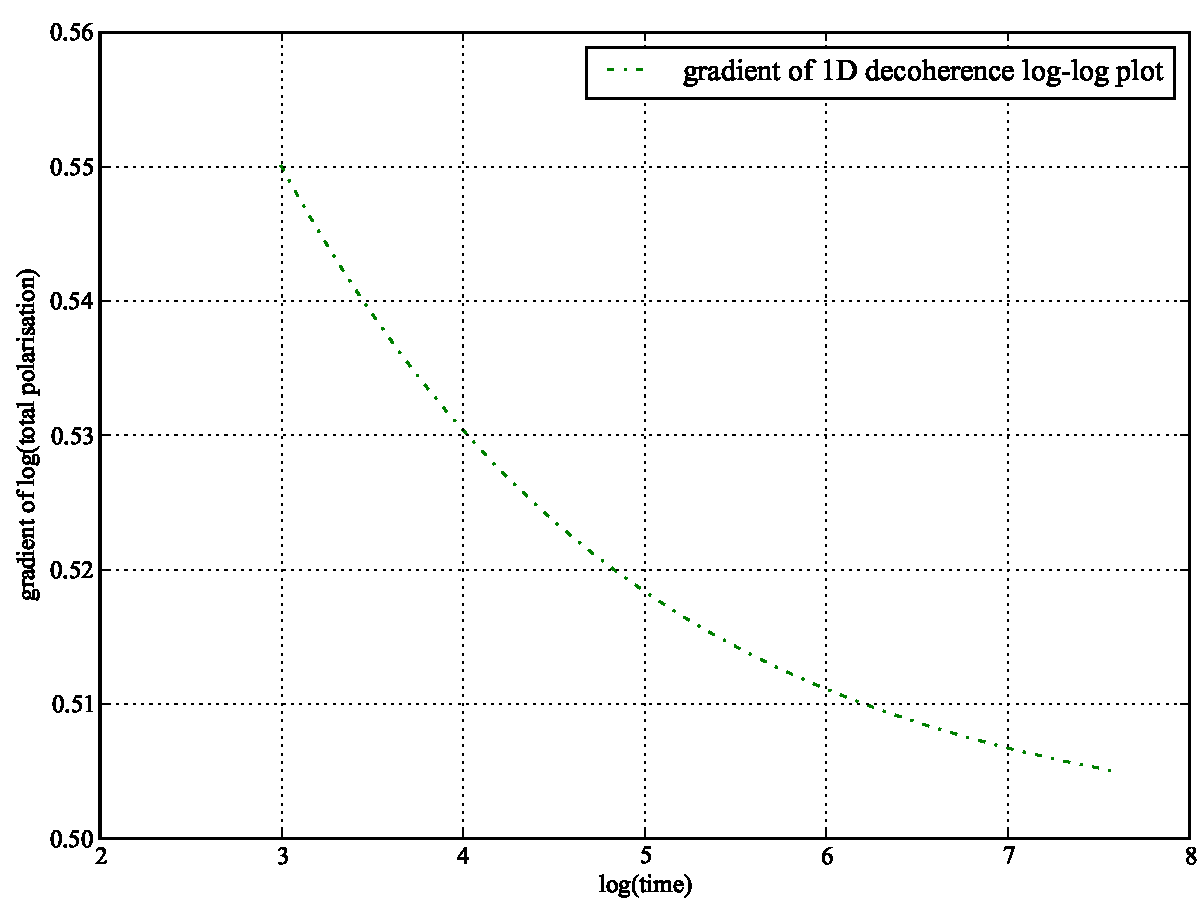
\includegraphics{assets/asymptotic_1d.pdf}
  \end{center}
  \caption{ The gradient of the `one dimension with decoherence' line tends to $\frac{1}{2}$ asymptotically.}
  \label{asymptotic_1d}
\end{figure}

In the two-dimensional case $g_{ij} = \sqrt{j}, j=i+1$: We get a random walk with increasing transition rates. Numerically (Fig. \ref{comparison}), we find that the rate of spin propagation drops from $t^2$ to $t$ - still an encouraging scaling.

        %%\subsection{Independent noise}

So far we considered a collective noise scenario, using a single Lindblad operator, $ L=\sum_{n}n\ket n\bra n$ . This is convenient to analyse for our system, as the system remains in the subspace covered by our basis of number states. A more realistic model involves treating the noise occurring at each site as independent. In this case we have Lindblad operators of the form
\begin{equation}
  L_i = \sigma_z^i
\end{equation}
for lattice sites $i$. Following a similar procedure to before we find the equivalent classical chain to be
\begin{equation}
  \dot{\rho}_{ii}=-\sum_{j\in
  P(i)}\frac{2|g_{ij}|^{2}}{\Gamma}\left(\rho_{ii}-\rho_{jj}\right)
  \label{qmat}
\end{equation}
where, crucially, the index now runs over all the partition states, rather than our basis of accessible states. In fact, in the 1D case these states are one and the same, and so the spin propagation goes as $\sqrt{t}$, as found in the collective noise case. In the 2D case, we are now performing a continuous-time classical random walk on Young's lattice. We are able to use the property that each node always has one more child than parents, to predict that the rate of spin propagation will be proportional to $t$ - the same as the collective noise case.  

\begin{figure}
  \begin{center}
    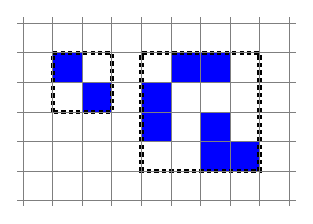
\includegraphics[scale=1]{assets/impurity}
  \end{center}
  \caption{Maximum extent of propagation of initialisation
    imperfections in the lattice - due to propagation rules
  imperfections are unable to grow beyond the dotted bounding boxes. }
  \label{impurities}
\end{figure}


\section{Robustness against Imperfect Initialisation}

Finally we consider imperfect inital polarisation (i.e. finite temperature) - a property exhibited by any real experimental system.  
A fortuitous consequence of the propagation rules is that our system is particularly robust against this source of error; it is difficult for imperfections in the centre of the lattice to spread (Fig. \ref{impurities}).

To estimate an upper bound for our initialisation threshold we took a randomly initialised lattice, with given imperfection probability, and evolved it using purely deterministic rules, to see whether the imperfections grew to cover over half the lattice. We expect this to give a loose upper bound for the quantum case, as quantum imperfections will both grow and shrink, making it less likely that they will compound in the same manner as deterministic growth. Fig \ref{flipthreshold} shows the results of these simulations; below $4\%$ the probability of growing to cover the majority of the lattice is negligible.
\begin{figure}[!h]
  \begin{center}
    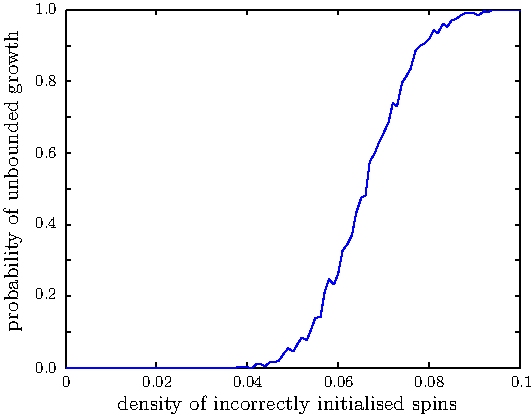
\includegraphics{assets/flipthreshold.pdf}
  \end{center}
  \caption{Probability that imperfections at given density will deterministically grow to cover over half the lattice.}
  \label{flipthreshold}
\end{figure}

This threshold places our protocol well within experimental capabilities; for example for an array placed in a standard W-band electron spin resonance system ($100$ GHz) and cooled using liquid 4He to $1.4$ degrees Kelvin, only $3.1\%$ of electron spins will be in the `up' state.

%\begin{acknowledgements}
%we thank gerard milburn and john morton for useful discussion. this work was supported by the epsrc, the national research foundation and ministry of education, singapore, and the royal society.
%\end{acknowledgements}
%\section{Conclusion}

%Although we know how the expected number of flipped spins increases with time, we have so far said nothing about how these spins are distributed throughout our sample. To investigate this we have plotted the value of the expected flipped spin density over the course of the evolution.  
%\begin{figure}[ht]
%  \begin{center}
%    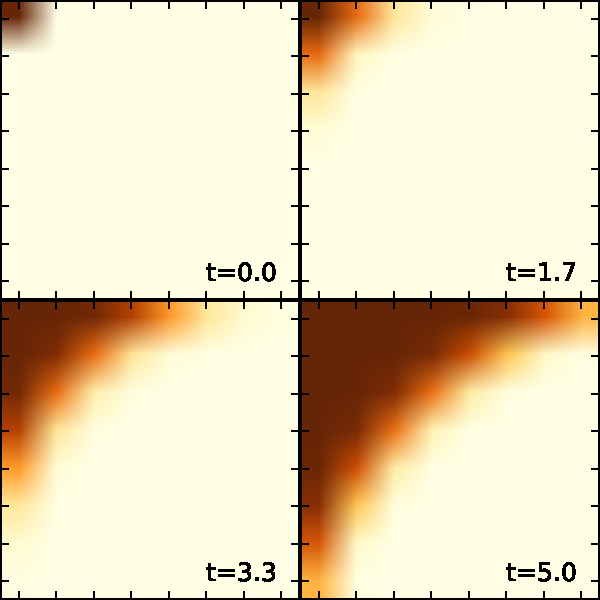
\includegraphics[scale =0.8] {assets/density_fig_all.pdf}
%  \end{center}
%  \caption{Density of flipped spins with time}
%  \label{densitypics}
%\end{figure}

%As you can see (Fig. \ref{densitypics} ), the area of high density is triangular in shape, of dimensions that scale linearly with the time elapsed. The boundary between areas of high and low density remains remarkably sharp, considering that the number state basis elements on which the motion is based have diffuse boundaries themselves.



\section{Conclusion}

Electron and nuclear spins have been employed in many of the early demonstrations of quantum technology but applications in real world QT are limited by the difficulty of measuring single spins. In this chapter we have shown that it is possible to rapidly and robustly amplify a spin state using a lattice of ancillary spins. The model we have employed corresponds to an extremely simple experimental system: a homogenous Ising-coupled spin lattice in one, two or three dimensions, driven by a continuous microwave field. We have constructed a natural basis for the problem and used this to assess the rate of amplification, both ideally and in the presence of environmental noise. We establish that the process can operate at finite temperature (imperfect initial polarisation) and under the effects of various forms of decoherence.
